\documentclass[10pt, twocolumn, twoside]{article}


\usepackage[left=1.15cm, right=1.15cm, top=1cm, bottom=0.9cm]{geometry}
\usepackage{graphicx} 
\usepackage{float}
\usepackage{titlesec}
\usepackage{amssymb,amsmath} 
\usepackage[euler]{textgreek}
\usepackage[backend=biber,style=numeric,sorting=ynt]{biblatex}
\usepackage{graphicx}
\usepackage{amsmath}
\usepackage{color}
\usepackage{listings}
\usepackage{bm}

\definecolor{dkgreen}{rgb}{0,0.6,0}
\definecolor{gray}{rgb}{0.5,0.5,0.5}
\definecolor{mauve}{rgb}{0.58,0,0.82}

% Settings for colour-coding and formatting Python code:
\lstset{
  language=Python,                % the language of the code
  basicstyle=\footnotesize,           % the size of the fonts that are used for the code
  numbers=left,                   % where to put the line-numbers
  numberstyle=\tiny\color{gray},  % the style that is used for the line-numbers
  stepnumber=5,                   % the step between two line-numbers. If it's 1, each line
                                  % will be numbered
  numbersep=5pt,                  % how far the line-numbers are from the code
  backgroundcolor=\color{white},      % choose the background color. You must add \usepackage{color}
  showspaces=false,               % show spaces adding particular underscores
  showstringspaces=false,         % underline spaces within strings
  showtabs=false,                 % show tabs within strings adding particular underscores
  frame=single,                   % adds a frame around the code
  rulecolor=\color{black},        % if not set, the frame-color may be changed on line-breaks within not-black text (e.g. commens (green here))
  tabsize=2,                      % sets default tabsize to 2 spaces
  captionpos=b,                   % sets the caption-position to bottom
  breaklines=true,                % sets automatic line breaking
  breakatwhitespace=false,        % sets if automatic breaks should only happen at whitespace
  title=\lstname,                   % show the filename of files included with \lstinputlisting;
                                  % also try caption instead of title
  keywordstyle=\color{magenta},          % keyword style
  commentstyle=\color{dkgreen},       % comment style
  stringstyle=\color{mauve},         % string literal style
  escapeinside={\%*}{*)},            % if you want to add LaTeX within your code
  morekeywords={*,...}               % if you want to add more keywords to the set
}

\addbibresource{name.bib}

\usepackage[colorlinks=true,linkcolor=blue]{hyperref}
\author{Alex WIlson\\Introduction to Statistical Methods}
\title{Exercise 1}

\date{\today}
\begin{document}

\maketitle %this uses the author, title, date information given in the preamble to make a title.

\begin{abstract}
The following is a report of fitting a data set to an Mth order polynomial using the least-squares method. Mth order polynomials have the general form
\begin{equation}
    f\left( x \right)=\sum_{i=1}^{M}\theta_{i}x^{i}
\end{equation}
\end{abstract}

\section{Plots}

\begin{table}[H]
\label{tab:data}
    \centering
    \begin{tabular}{|c|c|c|}
        \hline
        x &  y & $\sigma$ \\
        \hline
	    1.0	&	2.7 & 0.3	\\
	    2.0	&	3.9 & 0.5	\\
	    3.0	&	5.5 & 0.7	\\
	    4.0	&	5.8 & 0.6	\\
	    5.0	&	6.5 & 0.4	\\
	    6.0	&	6.3 & 0.3	\\
	    7.0	&	7.7 & 0.7	\\
	    8.0	&	8.5 & 0.8	\\
	    9.0 &   8.7 & 0.5   \\
        
        \hline
    \end{tabular}
    \caption{Dataset from course script\cite{script}. x-values controlled and have negligible uncertainty, and $\sigma$ is the standard deviation of y.}
    \label{tab:tabl}
\end{table}
Function defined in python, allowing for M=1,2,3

\begin{lstlisting}
def func(x,*theta):
    if M==3:
        theta0, theta1,theta2,theta3= theta
        return theta0 +theta1*x +theta2*x**2 + +theta3*x**3
    elif M==2:
        theta0, theta1,theta2= theta
        return theta0 +theta1*x +theta2*x**2
    elif M==1:
        theta0, theta1= theta
        return theta0 +theta1*x
\end{lstlisting}
\lstinline$*theta$ is a vector with an undetermined number of elements, allowing it to be changed, as shown in the above code, for any order of polynomials.

The method of least-squares is based on finding the value of $\overrightarrow{\theta}$ that minimises
\begin{equation}
    \chi^{2}( \theta)=\sum_{i,j=1}^{M}\frac{\left(y_{i}-f(x_{i};\overrightarrow{\theta})\right)^{2}}{\sigma_{i}^{2}}
\end{equation}
The value of $\overrightarrow{\theta}$ that minimises $\chi^{2}$ is $\hat{\theta}$.
Using \lstinline$curve.fit$ from \lstinline$scipy.optimise$ to get an estimation for $\hat{\theta}$, that can be used to plot a fit, based on how many starting points, \lstinline$p0$, and how many elements, $\overrightarrow{\theta}$, were given. Plots for M=1, M=2 and M=3 shown in plots \ref{fig:graph1}, \ref{fig:graph2}, \ref{fig:graph3}.
\begin{figure}
    \centering
    \centerline{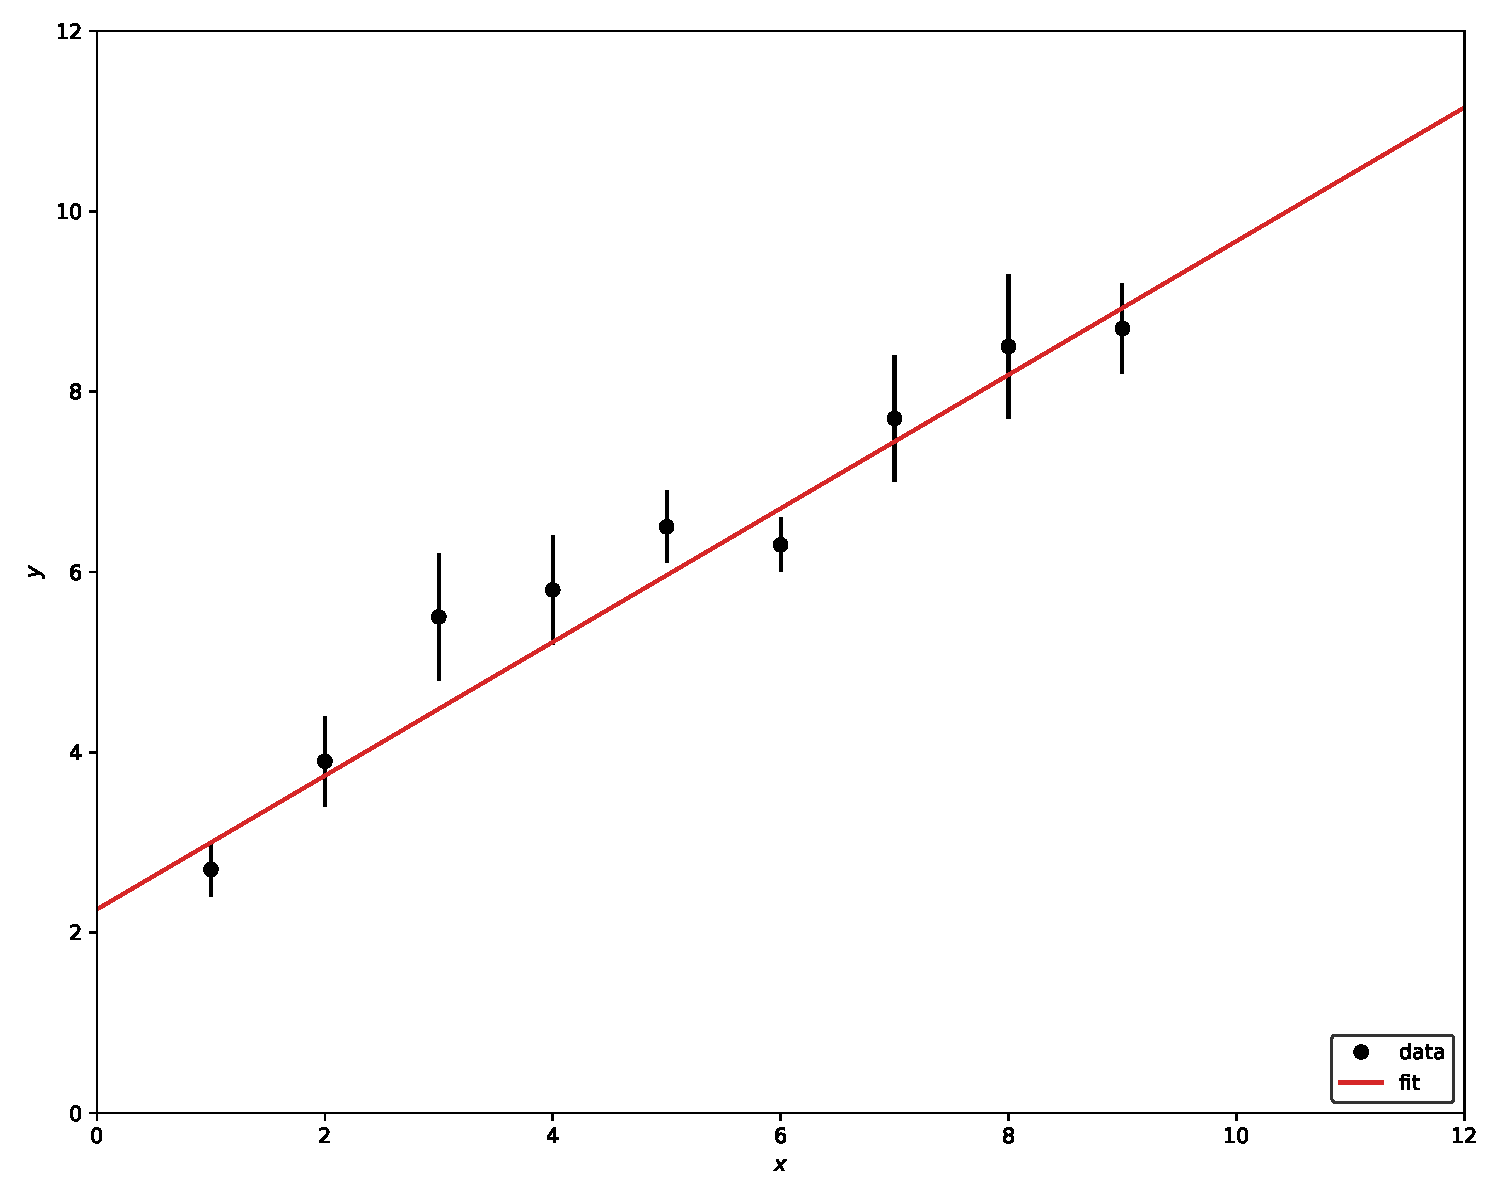
\includegraphics[scale=0.35]{Fitted Plot 1.pdf}}
    \caption{Straight-line (M=1) fit for data.}
    \label{fig:graph1}
\end{figure}
\begin{figure}
    \centering
    \centerline{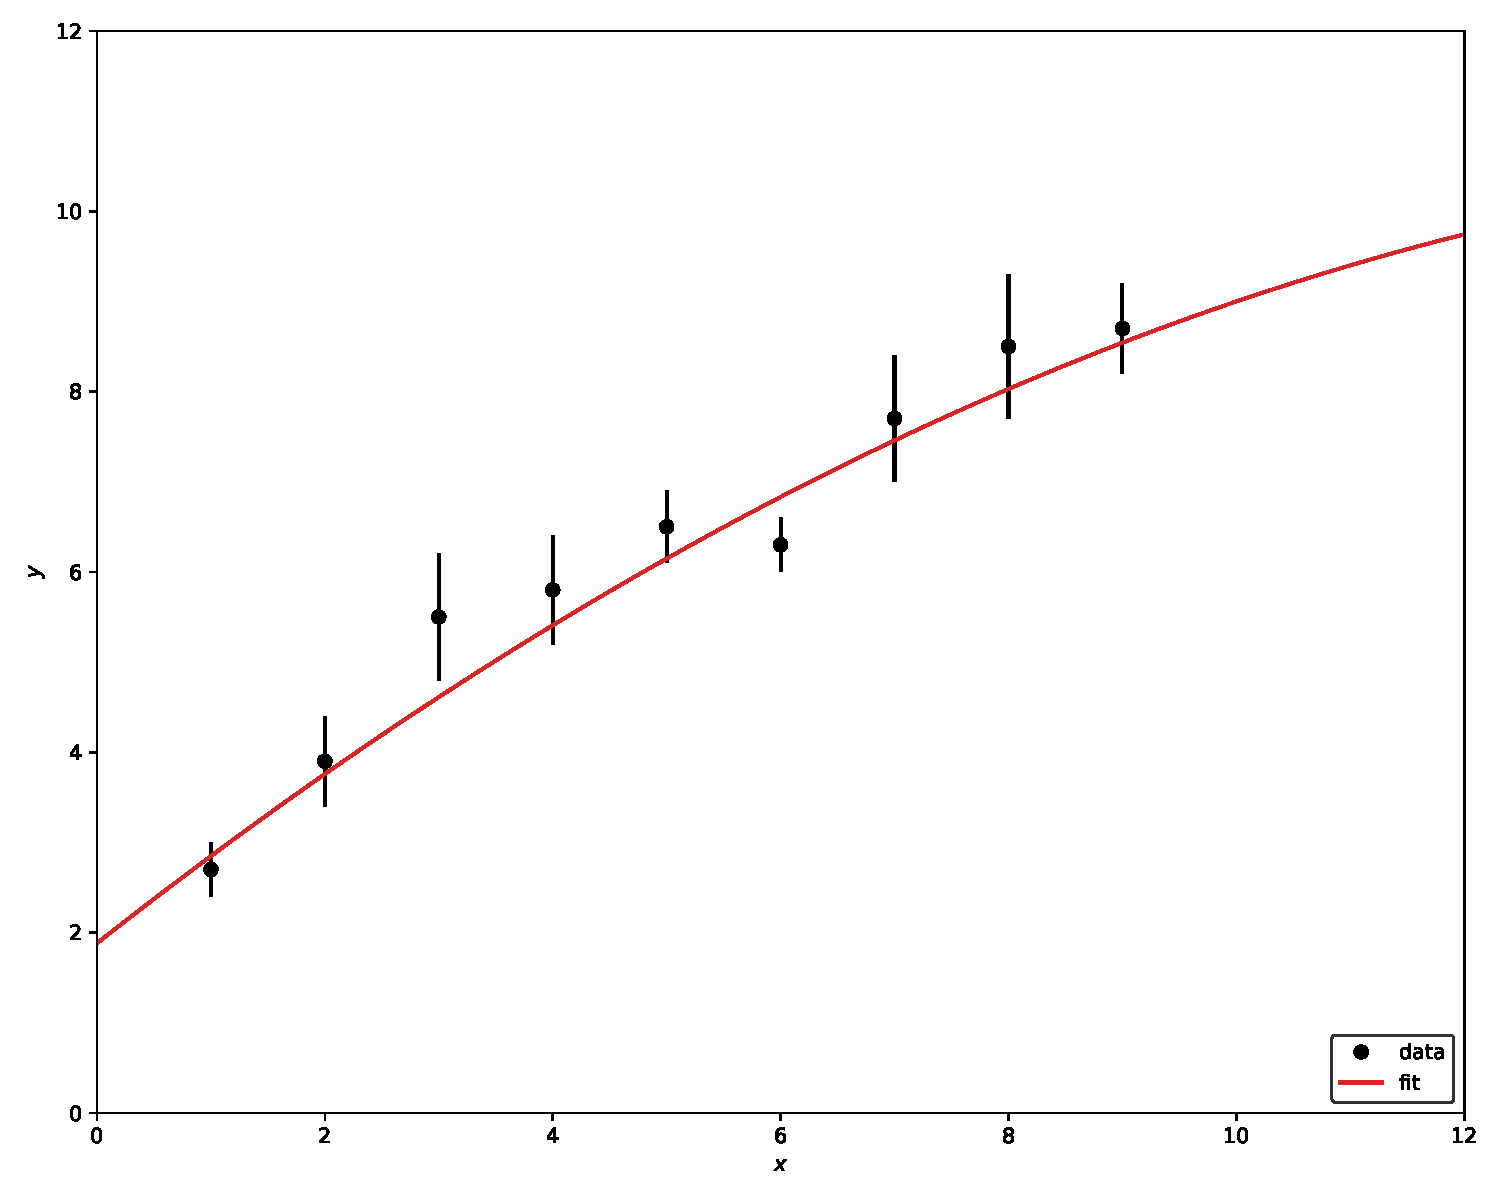
\includegraphics[scale=0.35]{Fitted Plot 2.pdf}}
    \caption{Straight-line (M=2) fit for data.}
    \label{fig:graph2}
\end{figure}
The \lstinline$curve.fit$ function outputs values for the fit parameters $\hat{\theta}$, as well as the covariance.
\begin{figure}
    \centering
    \centerline{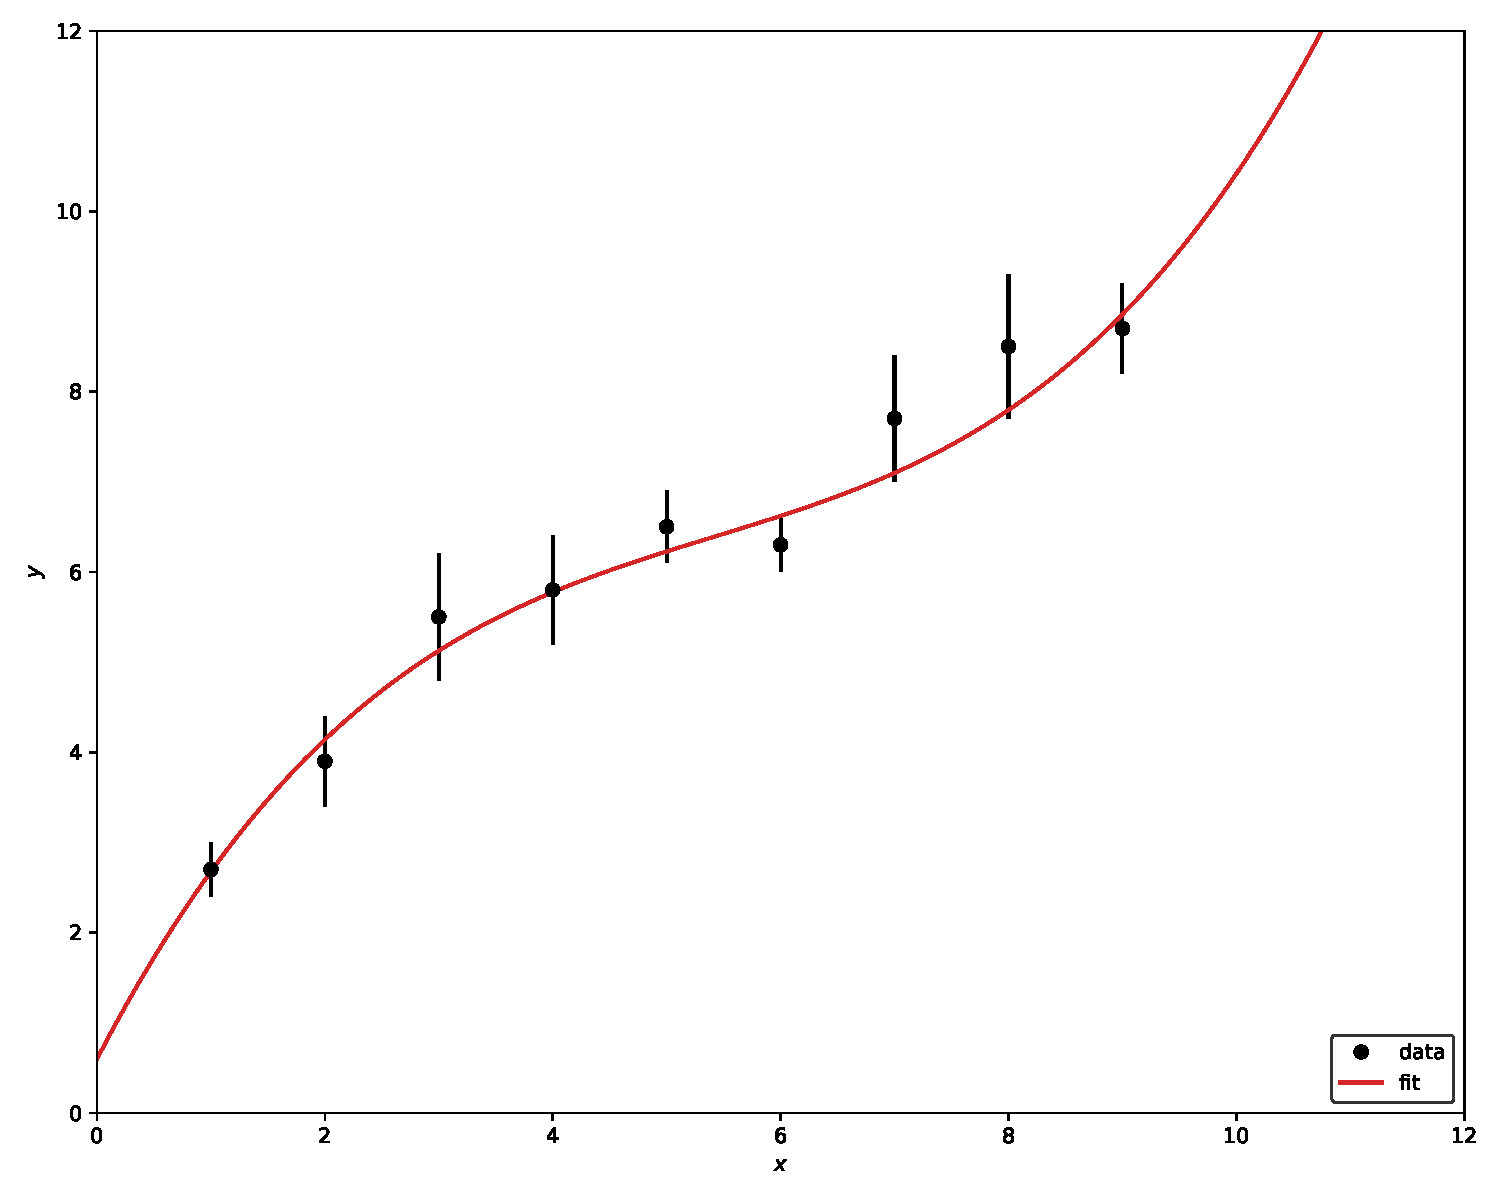
\includegraphics[scale=0.35]{Fitted Plot 3.pdf}}
    \caption{Cubic fit (M=3) fit for data.}
    \label{fig:graph3}
\end{figure}
The covariance given by the \lstinline$curve.fit$ function is then used to find the error in the fit using equation from the script \cite{script}
\begin{equation}
    \sigma^{2}\simeq \sum_{i=1}^{M}\frac{\partial u}{\partial \hat{\theta_{i}}}\frac{\partial u}{\partial \hat{\theta_{j}}}U_{ij}
\end{equation}
which can then be reduced to
\begin{equation}
    \sigma^{2} \simeq \sum_{i=1}^{M} x^{i+j}cov[i,j]
\end{equation}
that can be coded by defining this function
\begin{lstlisting}
def StDev(x,cov):
    k=[]
    z=[]
    for i in range(M+1):
        for j in range(M+1):
            k.append(x**(i+j)*cov[i,j])
    return (np.sqrt(sum(k)))
\end{lstlisting}
Then using \lstinline$fillbetween$ function from \lstinline$Matplotlib$ the errors in the fit can also be plotted, shown in \ref{fig:graph1a}, \ref{fig:graph2a}, \ref{fig:graph3a}.
\begin{figure}
    \centering
    \centerline{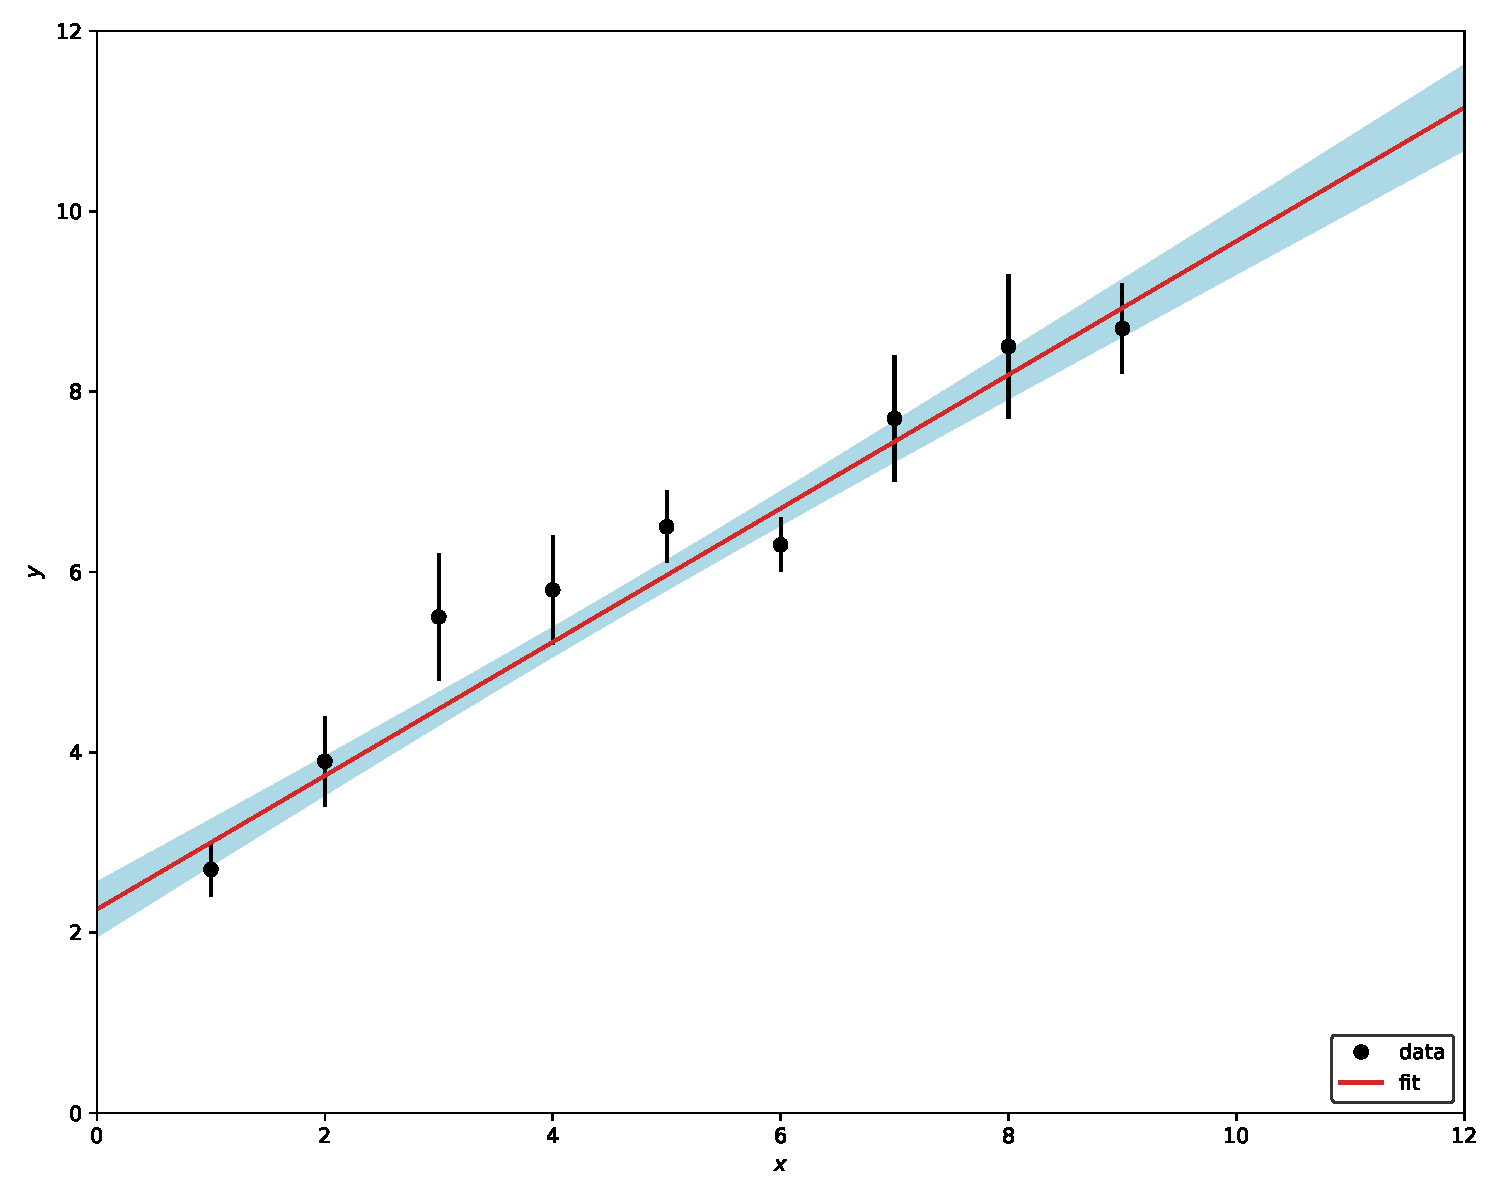
\includegraphics[scale=0.35]{Fitted Plot 1a.pdf}}
    \caption{Straight-line (M=1) fit for data, with error in fit shown in blue.}
    \label{fig:graph1a}
\end{figure}
\begin{figure}
    \centering
    \centerline{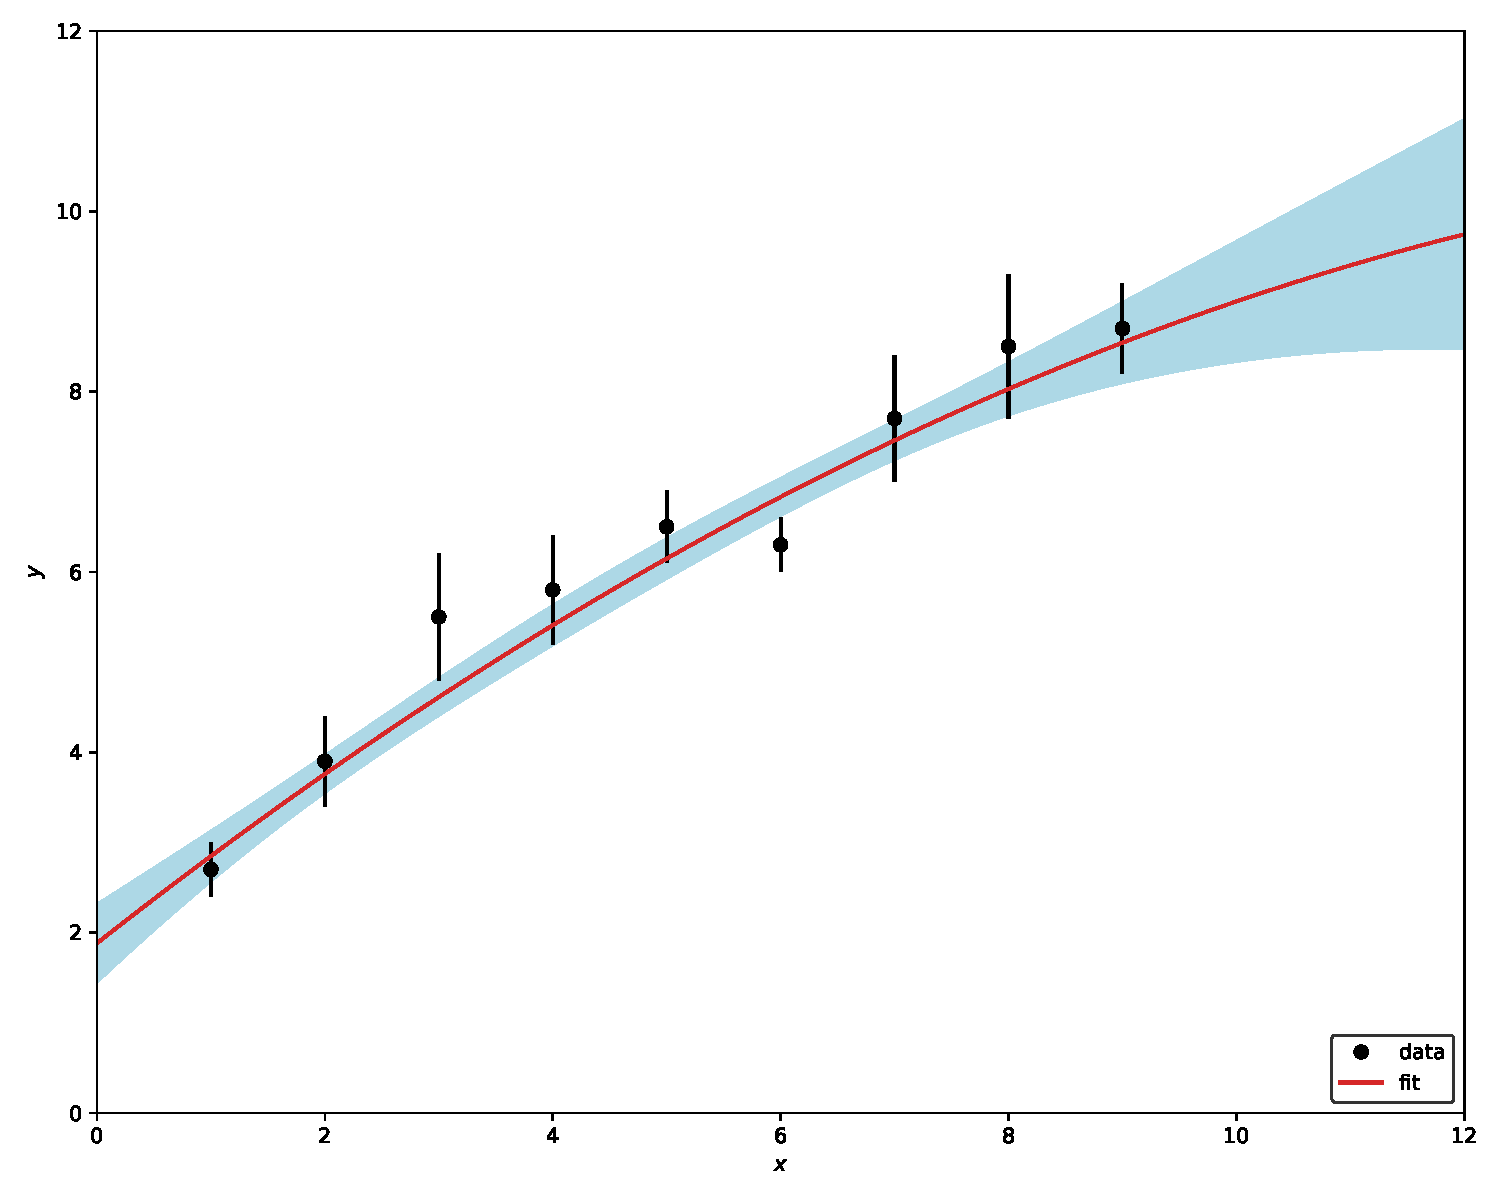
\includegraphics[scale=0.35]{Fitted Plot 2a.pdf}}
    \caption{Straight-line (M=2) fit for data, with error in fit shown in blue.}
    \label{fig:graph2a}
\end{figure}
\begin{figure}
    \centering
    \centerline{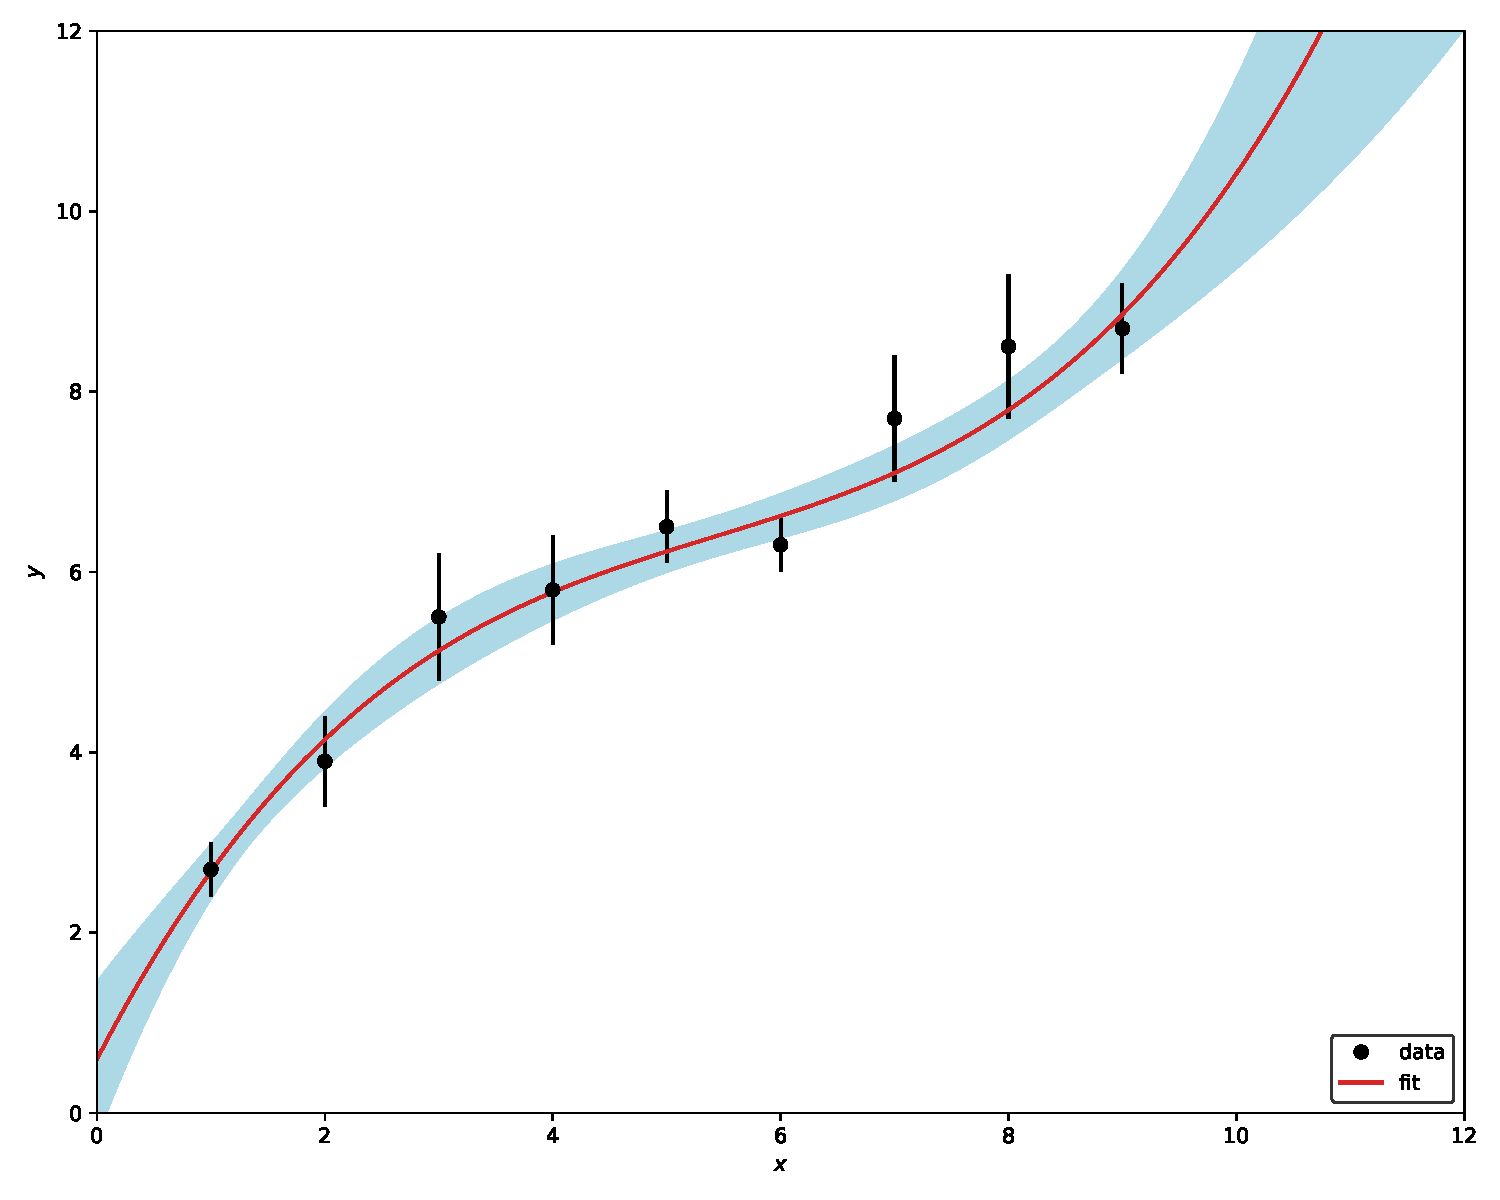
\includegraphics[scale=0.35]{Fitted Plot 3a.pdf}}
    \caption{Cubic fit (M=3) fit for data, with error in fit shown in blue.}
    \label{fig:graph3a}
\end{figure}





\begin{appendix}
\section{Python Code}\label{sec:python}
Code used to create plots shown below:
\lstinputlisting[language=Python,frame=single]{Exercise_1.py}
\end{appendix}

\printbibliography
\end{document}